% Section 4.3: The Systematics Stalemate
% Structure: Intro → NPTF Crisis → Morphological Ambiguity → DM Revival

\section{The Systematics Stalemate}
\label{sec:4.3}

The evidence reviewed in the preceding section, both for and against the MSP hypothesis, was obtained through template-based analyses that share a common vulnerability: their conclusions depend on modeling choices for which no unique, model-independent prescription exists.
The choice of interstellar emission model, the treatment of the Fermi Bubbles at low latitudes, the masking of known point sources, and the parameterization of the source-count function at the faint end each contribute irreducible systematic uncertainties that propagate into the final answer.
Over the past decade, a series of exchanges has demonstrated that these uncertainties are large enough to shift the conclusion between ``predominantly point sources'' and ``predominantly smooth emission'' depending on the analysis setup.
This section traces how the debate reached an impasse and how recent methodological advances are beginning to chart a path forward.

\subsection{The NPTF Crisis}
\label{sec:4.3.1}

The evidence for point sources presented in Section~\ref{sec:4.2.1} rested largely on the Non-Poissonian Template Fitting (NPTF) framework, which exploits the difference in photon statistics between smooth (Poissonian) emission and populations of unresolved point sources.
In 2019, a pair of analyses by Leane and Slatyer called the reliability of these results into question.

The first challenge came from a conceptually simple diagnostic: injecting a known, artificially generated dark matter signal into the real Fermi-LAT data and testing whether the NPTF pipeline could recover it~\cite{Leane:2019xiy}.
The injected signal was drawn from a Poisson distribution tracing a contracted NFW profile, exactly as expected from WIMP annihilation.
When the standard NPTF analysis was applied to this modified dataset, the injected dark matter flux was completely absorbed by the NFW point-source template, with the reconstructed dark matter component remaining consistent with zero.
This misattribution persisted even when the injected signal was scaled to a flux roughly five times larger than the GCE itself.
Only at injection levels approaching an order of magnitude above the observed excess did the fit begin to recover a dark matter component, and even then it returned only a fraction of the true injected value.

To understand the origin of this failure, Leane and Slatyer constructed a proof-of-principle simulation containing both a smooth dark matter signal and a population of point sources tracing the Fermi Bubbles.
When they deliberately excluded the Fermi Bubbles point-source template from the fit, leaving this population unmodeled, the NFW point-source template absorbed the mismodeled emission.
The simultaneously present dark matter signal was driven to zero, despite being the dominant component in the simulation.
This demonstrated that any unmodeled source population with a spatial morphology not fully degenerate with existing templates could fatally bias the NPTF, causing it to absorb and mask a genuine dark matter signal.

A deeper investigation followed in 2020, when Leane and Slatyer discovered a pronounced north-south asymmetry in the GCE~\cite{Leane:2020nmi,Leane:2020pfc}.
Within a $10^\circ$ region of interest, the smooth excess in the northern hemisphere was found to be substantially brighter than in the south, with the data preferring this asymmetric model at enormous statistical significance (Bayes factors up to $\sim 10^{27}$ in favor of asymmetry).
As shown analytically in their companion paper~\cite{Leane:2020pfc}, an overly rigid symmetric template that cannot capture this spatial variance in the data will generate excess pixel-to-pixel scatter that the NPTF interprets as point-source emission.
When the authors subdivided the GCE template into independent northern and southern components and allowed both to float freely, the flux attributed to the point-source templates dropped to values consistent with zero.
The Bayes factor in favor of point sources, which had stood at $\sim 10^{15}$ under the assumption of a symmetric GCE, collapsed by fourteen orders of magnitude to less than 10, rendering the preference for point sources statistically negligible.

These results did not go unchallenged.
Buschmann et al.~\cite{Buschmann:2020adf} argued that the signal injection failures reported by Leane and Slatyer were driven primarily by the use of the older \texttt{p6v11} Galactic diffuse emission model, which suffers from severe over-subtraction in the inner Galaxy.
In this model, the diffuse template absorbs more flux than it should, driving the smooth GCE normalization to unphysical negative values and creating a mathematical ``hole'' that swallows any injected dark matter signal before it can be recovered.
To address this, Buschmann et al.
\ introduced several improvements: a state-of-the-art hydrodynamic diffuse model (Model~O) that provided a substantially better fit to the data; a spherical-harmonic marginalization technique that corrects for large-scale mismodeling in a data-driven manner without erasing small-scale structure; and a truncated source-count function that conservatively excludes point sources below the one-photon detection threshold, thereby breaking the mathematical degeneracy between ultra-faint sources and smooth emission~\cite{Chang:2019ars}.
With these modifications, the signal injection test worked correctly (injected dark matter signals were properly recovered), yet the data still yielded a Bayes factor of $\sim 10^{3.4}$ in favor of point sources.
Similar conclusions were reached independently by Calore et al.~\cite{Calore_2021} using the 1-point Probability Density Function (1pPDF) technique. The 1pPDF is an analytical framework mathematically equivalent in its goals to the NPTF, leveraging pixel-count statistics to reconstruct the source-count distribution. By combining 1pPDF with adaptive template fitting, they demonstrated that point sources constitute a robust sub-threshold component of the GCE, provided the diffuse emission is accurately modeled.

The exchange exposed a fundamental tension: the NPTF results depend sensitively on analysis choices that remain debatable.
% The preference for point sources can be made to appear or vanish depending on the diffuse model, the treatment of spatial asymmetries, and the parameterization of the source-count function at the faint end.
\blue{The preference for point sources can be made to appear or vanish depending on the diffuse model, the treatment of spatial asymmetries, and the other modeling choices enumerated at the opening of this section.}
No analysis to date has achieved a resolution that all groups accept, and the community consensus has shifted accordingly: the NPTF, as currently implemented, cannot robustly distinguish between smooth and point-source emission in the inner Galaxy.

\subsection{The Morphological Ambiguity}
\label{sec:4.3.2}

Beyond the statistical question of smooth versus point-source emission, the spatial morphology of the GCE itself has become a second axis of contention.
As discussed in Section~\ref{sec:4.1.3}, the excess was initially characterized as approximately spherically symmetric, centered on Sgr~A$^*$, and consistent with a generalized NFW profile with inner slope $\gamma \approx 1.1$--$1.3$.
This morphology has no obvious astrophysical counterpart among known Galactic structures and was therefore regarded as a strong indicator of dark matter annihilation.
% However, a series of analyses beginning with Macias et al.~\cite{Macias:2016nev,Macias:2019omb} and Bartels et al.~\cite{Bartels:2017vsx} challenged this picture by arguing that the GCE traces the boxy, X-shaped stellar bulge of the Milky Way rather than a smooth, spherically symmetric halo.
% Using near-infrared stellar mass maps as spatial templates, these studies found that the stellar bulge template absorbed the GCE flux with a statistically better fit than a standard NFW profile, supporting an astrophysical origin tied to the old stellar population of the inner Galaxy.
\blue{However, the stellar-bulge template analyses of Macias et al.~\cite{Macias:2016nev,Macias:2019omb} and Bartels et al.~\cite{Bartels:2017vsx}, introduced in Section~\ref{sec:4.2.1}, challenged this picture by finding that the boxy, X-shaped stellar bulge fits the GCE better than a spherically symmetric NFW halo.}

The significance of this claim, however, depends sensitively on the analysis setup.
% Whether the GCE prefers an NFW or bulge morphology can shift depending on the interstellar emission model adopted, the masking procedure applied to the Galactic plane and known point sources, and how the Fermi Bubbles emission is treated at low latitudes~\cite{Macias:2019omb,Cirelli:2024ssz}.
\blue{Whether the GCE prefers an NFW or bulge morphology can shift depending on the same diffuse-emission systematics discussed at the opening of this section~\cite{Macias:2019omb,Cirelli:2024ssz}.}
Because the true diffuse background in the inner Galaxy is not known to the precision required, the template fitting procedure is inherently subject to systematic uncertainties that propagate directly into the morphological inference.
Different groups, using equally defensible analysis choices, have reached opposite conclusions: some find a strong preference for the bulge template, while others recover a spherically symmetric signal fully consistent with dark matter.
No interstellar emission model achieves statistical fluctuation-level agreement with the data in the inner Galaxy; persistent large-scale residuals remain regardless of the morphological template adopted for the GCE.
As a result, all morphological conclusions drawn from current analyses should be regarded as provisional.

Beyond the morphological debate, which remains unresolved at the spatial level, an independent spectral observation further complicates the astrophysical interpretation.
Cholis et al.~\cite{Cholis:2021rpp} examined the high-energy behavior of the GCE spectrum above $\sim 10$~GeV and found emission extending well beyond the energies at which millisecond pulsars are expected to contribute.
The gamma-ray spectra of known MSPs exhibit exponential cutoffs at a few GeV, a characteristic feature of curvature radiation in pulsar magnetospheres.
The presence of a power-law tail at higher energies is difficult to reconcile with a purely MSP origin and suggests that either a second emission component contributes at high energies or that the GCE is not entirely astrophysical.
This spectral argument operates independently of the morphological debate and was initially cited as evidence against a complete MSP explanation.

However, this high-energy argument has recently been directly challenged.
Manconi et al.~\cite{manconi2024galacticcenterexcesshighest} extended the 1pPDF technique to the $>10$~GeV regime, combining it with adaptive template fitting to evaluate both the morphology and the photon-count statistics of the high-energy tail.
They found strong evidence for the GCE at these elevated energies, noting that the emission strongly prefers a bulge morphology over a dark matter template.
Crucially, their 1pPDF analysis reconstructed a significant population of faint, sub-threshold point sources at these high energies.
% This provides robust evidence that the high-energy tail of the GCE can be explained by a population of point sources---likely MSPs with harder spectra or a distinct sub-population---rather than requiring a dark matter contribution or an exotic secondary component.
\blue{Manconi et al.\ interpret this as evidence that the high-energy tail of the GCE can be explained by a population of point sources---possibly MSPs with harder spectra or a distinct sub-population---without requiring a dark matter contribution or an exotic secondary component.}

Taken together, the morphological and spectral ambiguities reinforce the conclusion that the current generation of template-based analyses cannot definitively identify the source of the GCE.
% The answer depends on modeling choices for which there is no clear, model-independent criterion to adjudicate.
\blue{It is precisely this impasse that motivates the energy-dependent inference discussed in Section~\ref{sec:4.3.3} and the independent constraints, obtained far from the Galactic Center, that we develop in Section~\ref{sec:4.4}.}

\subsection{Recent Revival of the Dark Matter Hypothesis}
\label{sec:4.3.3}

While the debates over the NPTF and the GCE morphology exposed deep vulnerabilities in established methods, a recent analysis has reframed the question entirely by incorporating energy information into the point-source inference for the first time.
List et al.~\cite{List:2025qbx} developed a CNN-based simulation-based inference framework that simultaneously fits the spatial and spectral properties of the inner Galaxy across ten logarithmically spaced energy bins from 2 to 20~GeV.
Unlike the original NPTF, which discarded all spectral information and neglected pixel-to-pixel correlations from the finite point-spread function, this approach exploits the fact that the GCE has a distinct energy spectrum from the dominant diffuse backgrounds, providing an additional lever arm to separate signal from astrophysical contamination (see Chapter~\ref{ch:methods} for background on simulation-based inference).

The inclusion of energy information substantially alters the inferred source-count distribution (SCD).
% Earlier analyses, both the 2016 NPTF~\cite{Lee:2015fea} and energy-independent CNN approaches~\cite{List:2020mzd}, had placed the hypothetical point-source population near or just below the Fermi detection threshold, typically predicting populations of a few hundred sources (the 2016 NPTF preferred approximately 200).
\blue{Earlier analyses, both the 2016 NPTF~\cite{Lee:2015fea} and energy-independent CNN approaches~\cite{List:2020mzd}, had placed the hypothetical point-source population near or just below the Fermi detection threshold, typically predicting populations of a few hundred sources --- from $\sim 260$ when resolved catalog sources are masked to the $\sim 400$ quoted in Section~\ref{sec:4.2.1} when they are not~\cite{Lee:2015fea}.}
The energy-dependent CNN drives the SCD to far fainter fluxes: the inferred distribution resides almost entirely below the one-photon threshold, meaning that a typical source would not even produce a single detected photon.
To account for the total observed GCE flux with such faint sources, the median prediction requires approximately 200{,}000 sources, with a 90\% confidence lower bound of roughly 35{,}000~\cite{List:2025qbx}.

\begin{figure}[t]
	\centering
	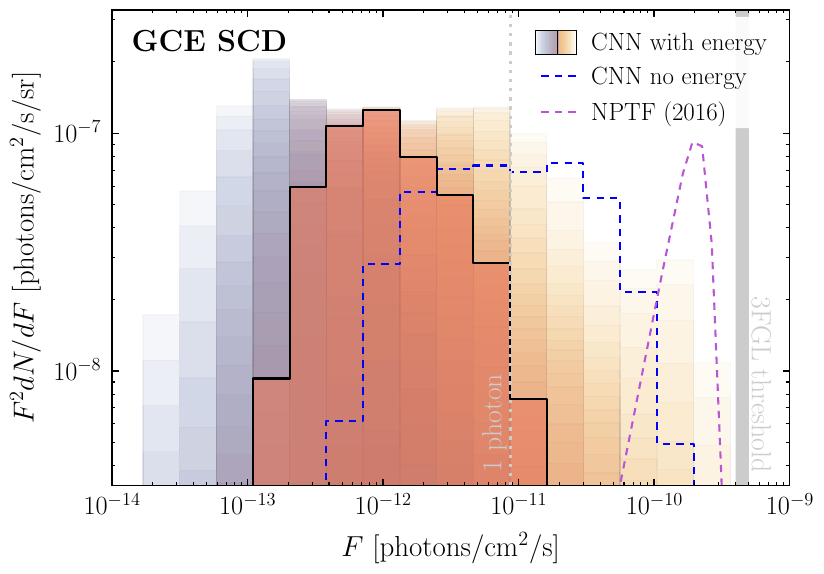
\includegraphics[width=0.7\columnwidth]{figures/List2025_fig1_scd.png}
	\caption{Source-count distribution (SCD) of the GCE inferred via three approaches.
		The NPTF (dashed purple) placed the emission just below the Fermi 3FGL detection threshold; an energy-independent CNN (dashed blue) preferred a somewhat fainter population.
		Including energy information (solid black, with quantile bands from purple to orange) drives the SCD below the one-photon line.
		At this level, at 95\% confidence, only 3\% of the emission can be excluded as Poissonian.
		From \cite{List:2025qbx}, Figure~1 (right panel).
	}
	\label{fig:gce_scd}
\end{figure}

This result has a fundamental consequence.
A population of point sources so faint that individual members produce fewer than one detected photon is mathematically indistinguishable from smooth, Poissonian emission, which is exactly the spatial signature predicted by dark matter annihilation.
The distinction between the point-source and dark matter hypotheses is a nested one: an infinite number of infinitely dim sources produces exactly Poisson statistics.
To quantify how much of the GCE can actually be attributed to point sources, List et al.
\ trained a dedicated neural network to distinguish Poissonian from point-source emission given the inferred SCD.
For the median SCD prediction, at 95\% confidence only 3\% of the GCE emission can be excluded as having a Poissonian origin~\cite{List:2025qbx}.
The remaining 97\% is fully consistent with the smooth emission expected from dark matter.
This represents a marked shift from the earlier energy-independent CNN analysis, which had been able to exclude 34\% of the emission as Poissonian at the same confidence level.
\blue{This consistency reopens the dark matter hypothesis, but it does not demonstrate it: the result removes an obstacle to a smooth-emission origin rather than establishing one.}

The implications are twofold.
First, the key historical evidence that the GCE originates from point sources, including the NPTF's strong Bayes factor and the inferred SCD peaking near the detection threshold, is substantially weakened when spectral information is properly incorporated.
Second, if the GCE is nonetheless produced by astrophysical point sources, those sources must be extraordinarily faint and numerous, forming a population with no direct precedent among known Galactic source classes.
As we will discuss in Section~\ref{sec:4.4}, this ultra-faint regime is precisely where independent constraints from globular cluster observations become most informative: the MSP luminosity function measured in globular clusters predicts sources that are far too bright and too few to match the distribution required by the energy-dependent analysis.
